\documentclass[12pt]{report}
\usepackage[utf8]{inputenc}
\usepackage{graphicx}
\graphicspath{{images/}}
\usepackage[a4paper,width=150mm,top=25mm,bottom=25mm]{geometry}
\usepackage{listings}
\usepackage{pythonhighlight}
\usepackage{caption}
\usepackage{subcaption}
\usepackage[sorting=ydnt]{biblatex}
\usepackage{amsmath}
\usepackage{tikz}
\usepackage{mathdots}
\usepackage{yhmath}
\usepackage{cancel}
\usepackage{color}
\usepackage{siunitx}
\usepackage{array}
\usepackage{multirow}
\usepackage{amssymb}
\usepackage{tabularx}
\usepackage{extarrows}
\usepackage{booktabs}
\usetikzlibrary{fadings}
\usetikzlibrary{patterns}
\usetikzlibrary{shadows.blur}
\usetikzlibrary{shapes}
\usepackage{tikz}
\usetikzlibrary{shapes.geometric, arrows}
\tikzstyle{startstop} = [rectangle, rounded corners, minimum width=3cm, minimum height=1cm,text centered, draw=black, fill=red!30]
\tikzstyle{process} = [rectangle, minimum width=3cm, minimum height=1cm, text centered, text width=3cm, draw=black, fill=orange!30]
\tikzstyle{io} = [trapezium, trapezium left angle=70, trapezium right angle=110, minimum width=3cm, minimum height=1cm, text centered, draw=black, fill=blue!30]
\tikzstyle{process} = [rectangle, minimum width=3cm, minimum height=1cm, text centered, draw=black, fill=orange!30]
\tikzstyle{decision} = [diamond, minimum width=3cm, minimum height=1cm, text centered, draw=black, fill=green!30]
\tikzstyle{arrow} = [thick,->,>=stealth]

\addbibresource{references.bib} 

\title{
    {Using Autocorrelation to identify a representative cycle in a larger dataset with Python}\\\
    
    {\large Loughborough University - Wolfson School of Engineering}\\\

    {
\includegraphics[width=70mm,scale=0.5]{university.png}}\\\
    
    {\large Caterpillar Inc. – Research department}\\\
    
    {
\includegraphics[width=70mm,scale=0.5]{caterpillar.png}}
    
}

\author{Tomás Apolónia}

\date{April 2022}

\begin{document}
\maketitle
\tableofcontents

\chapter{Introduction}
\raggedright
\section{Background and context to the problem}
Finding useful information in vast amount of data is as difficult as `finding a needle in a haystack'. Using \textbf{automated} statistical tools to analyse these large data sets can provide valuable information to assist decision making.

Context to the problem the report is trying to solve. When a CAT machine finishes field testing, it has recorded over 100 channels of data for each test run. An example of a run could include lifting a bucket of sand and unloading it onto a truck. This action is repeated multiple times by the operator throughout a test. Consequently, a \textbf{pattern} emerges in every data channel due to this repeated action. The \textbf{pattern} is the bases of this report. If the operator did not repeat any actions, the tool would not be applicable. 
Using the author's tool, Engineers can now efficiently analyse this much data. 

\textbf{Cycle}:

A snippet of time is extracted from the larger dataset. In the report's case, the extracted data is roughly 30 to 120 seconds in length (the duration of the repeated task). The extracted data is called a "CYCLE" throughout this report.

\section{What sort of data is suitable?}
A suitable data source can range from a street's foot traffic during one day to the strain force of a boom arm on an excavator. 
The perfect case scenario is time series data with low noise and randomness but high repeatability. Using data that has 10+ cycles improves the filtering and selection process shown in \ref{filtering}. Unsuitable data is high noise and randomness with a total cycle count below five. 

The tool is unaffected by the length of the dataset but highly affected by the total repeated cycles in a dataset. Aim for five minimum cycles. More on limitations will be talked about in \ref{limitation}.

The Datasets in this report include three separate files of CAT Machine data with varying magnitudes, randomness and noise. Shown in Figure \ref{data table}

\begin{figure}
\begin{tabular}{|l|l|l|l|}
\hline
\textbf{Dataset}                                                      & \textbf{A}                                                            & \textbf{B}                                                                        & \textbf{C}                                                                      \\ \hline
\textbf{Description}                                                  & \begin{tabular}[c]{@{}l@{}}Displacement Tilt \\ cylinder \end{tabular} & \begin{tabular}[c]{@{}l@{}}Displacement Steering \\ cylinder\end{tabular} & \begin{tabular}[c]{@{}l@{}}Force Strain gauge \\ steering cylinder\end{tabular} \\ \hline
\textbf{\begin{tabular}[c]{@{}l@{}}Length of \\ dataset\end{tabular}} & 20 mins                                                                & 20 mins                                                                    & 20 mins                                                                          \\ \hline
\end{tabular}
\caption{Datasets}
\label{data table}
\end{figure}



\subsection{Time series data vs  non-time series data?}
Time series data are sequential (ordered by timestamp) and have constant time intervals between data points. In other words, data collected by an event-based data collection system are not time series unless events happen deterministically at constant time intervals.

A rule of thumb to identify the data you received is, does the data comes with timestamps alongside the magnitude values? Time series. The exception to this rule, is data that is only 1 attribute \textit{but} includes the frequency.
To derive the timestamps from single attribute data using frequency is shown in Figure \ref{frequency table}

\begin{figure}
\centering
\begin{tabular}{c|c|c}
\textbf{Row nº} & \textbf{Magnitude} & \textbf{\begin{tabular}[c]{@{}c@{}}Resulting \\ Time stamp \\ \end{tabular}} \\ \hline
0 & -1.243801  & 0/500 = 0   \\
1 & -1.103403  & 1/500 = 0.002 \\
2 & -0.9631792 & 2/500 = 0.004 \\
3 & -0.9158725 & 3/500 = 0.006 \\
... & ... & ... \\
13750 & -1.122155 & 13750/500 = 27.5
\end{tabular}
\[f = \frac{rev}{t}\]
\caption{Frequency table Dataset C, 500hz}
\label{frequency table}
\end{figure}




\chapter{Background literature review}
\section{How does Autocorrelation work?}
Autocorrelation is matching a signal compared to a delayed version of itself. This delay between the original signal and the delay is called ‘lag'. 

``The autocorrelation \cite{Jenkins} function can be used for the following two purposes:

\begin{itemize}

    \item To detect non-randomness in data.
    
    \item To identify an appropriate time series model if the data are not random.
    
\end{itemize}

Given measurements, Y1, Y2, ..., YN at time X1, X2, ..., XN, the lag k autocorrelation function is defined as
\begin{figure}[h]
\centering

\begin{math}
{ {r_{k} = \frac{\sum_{i=1}^{N-k}(Y_{i} - \bar{Y})(Y_{i+k} -  \bar{Y})} {\sum_{i=1}^{N}(Y_{i} - \bar{Y})^{2} }} }
\end{math}

\caption{Autocorrelation Formula}
\label{autocorrolationF}
\end{figure}

Although the time variable, X, is not used in the formula for Autocorrelation, the assumption is that the observations are equispaced.

Autocorrelation is a correlation coefficient. However, instead of a correlation between two different variables, the correlation is between two values of the same variable at times Xi and Xi+k.

In our case we use Autocorrelation to identify an appropriate time series model, hence we plot with many lags." \cite{NIST}

\subsection{How does this apply?}

The Autocorrelation coefficient has now been explained mathematically, but how is this shown graphically? 
Looking at Figure \ref{ACF coefficient}, starting on the Y axis. The scale goes from -1 to 1, 1 = 100\% match while 0 = 0\% correlated. X axis's being the datapoints. These peaks seen on the graph is what the script looks for when identifying representative cycles. 
\begin{figure}[h]
\centering
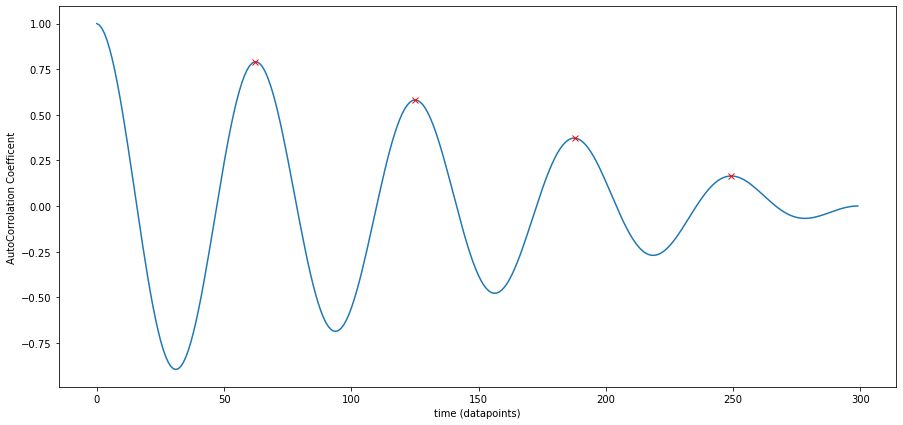
\includegraphics[scale=0.45]{images/ACF u DIAGRAM.png}
\caption{ACF tutorial}
\label{ACF coefficient}
\end{figure}

\section{Other methods of pattern recognition}
This research section is in chronological order. Before diving into the different types of pattern recognition and approaches. All methods need to follow this approach to be considered. Using work produced by paper \cite{DBLP:journals/corr/abs-2104-07406}, a table was made for time series data, allowing users to filter by task required, e.g. forecasting,	classification,	clustering,	anomaly detection... Below are is a list of all the libraries that fit the reports need ``pattern recognition".

\tikzset{every picture/.style={line width=0.75pt}} %set default line width to 0.75pt        


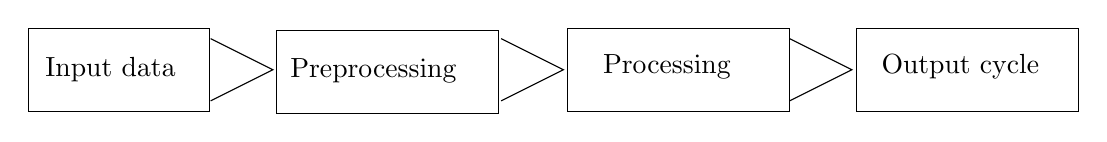
\begin{tikzpicture}[x=0.75pt,y=0.75pt,yscale=-1,xscale=1]
%uncomment if require: \path (0,300); %set diagram left start at 0, and has height of 300

%Shape: Rectangle [id:dp6164774614967738] 
\draw   (88.14,122) -- (175.44,122) -- (175.44,162) -- (88.14,162) -- cycle ;
%Shape: Rectangle [id:dp8360875880221361] 
\draw   (207.63,123) -- (314.63,123) -- (314.63,163) -- (207.63,163) -- cycle ;

%Shape: Rectangle [id:dp6039686166404709] 
\draw   (347.82,122) -- (454.82,122) -- (454.82,162) -- (347.82,162) -- cycle ;

%Shape: Rectangle [id:dp467126276166151] 
\draw   (487,122) -- (594,122) -- (594,162) -- (487,162) -- cycle ;

\draw   (176,127) -- (206,142) -- (176,157) ;
\draw   (316,127) -- (346,142) -- (316,157) ;
\draw   (455,127) -- (485,142) -- (455,157) ;

% Text Node
\draw (213.13,135.5) node [anchor=north west][inner sep=0.75pt]   [align=left] {Preprocessing};
% Text Node
\draw (363.82,133.5) node [anchor=north west][inner sep=0.75pt]   [align=left] {Processing};
% Text Node
\draw (498,133.5) node [anchor=north west][inner sep=0.75pt]   [align=left] {Output cycle};
% Text Node
\draw (95.17,134.5) node [anchor=north west][inner sep=0.75pt]   [align=left] {Input data};

\end{tikzpicture}

\subsection{Stumpy}
On 17 Jul 2019, stumpy library was created. This library was born from the essential research created by the  University of New Mexico, Riverside and the University of California. ``described an exact method called STOMP for computing the matrix profile for any time series with a computational complexity of O(n2)!" \cite{law2019stumpy} 

\subsubsection{Matrix profile} ``At its core, the STUMPY library efficiently computes something called a matrix profile, a vector that stores the z-normalized Euclidean distance between any subsequence within a time series and its nearest neighbour." ``...With the academics, data scientists, and developers in mind, we have taken these concepts and have open sourced STUMPY, a powerful and scalable library that efficiently computes the matrixprofile according to this published research." \cite{law2019stumpy}. If the reader wants to dive deeper into the details of z-normalized Euclidean distance. Read the winner of the best paper award ICDM 2017. \cite{zhu_imamura_nikovski_keogh_2017}.

\subsubsection{How can Stumpy be implemented for pattern recognition?}
Utilizing dataset A with STUMP function, the graphs in Figure: \ref{Motif} were produced.
The Y axis is the z-normalized Euclidean distance shown on the bottom plot. The higher this value, the lower the ``correlation". This is illustrated by the best cycles selected starting at the lowest points on the Matrix profile.

To automatically select the lowest point on the Matrix profile, a NumPy sorting algorithm is used to select the first point.

\begin{python}
motif_idx = np.argsort(mp[:, 0])[0]
print(f"The motif is located at index {motif_idx}")
\end{python}
The motif is located at index 85062

\begin{figure}
\centering
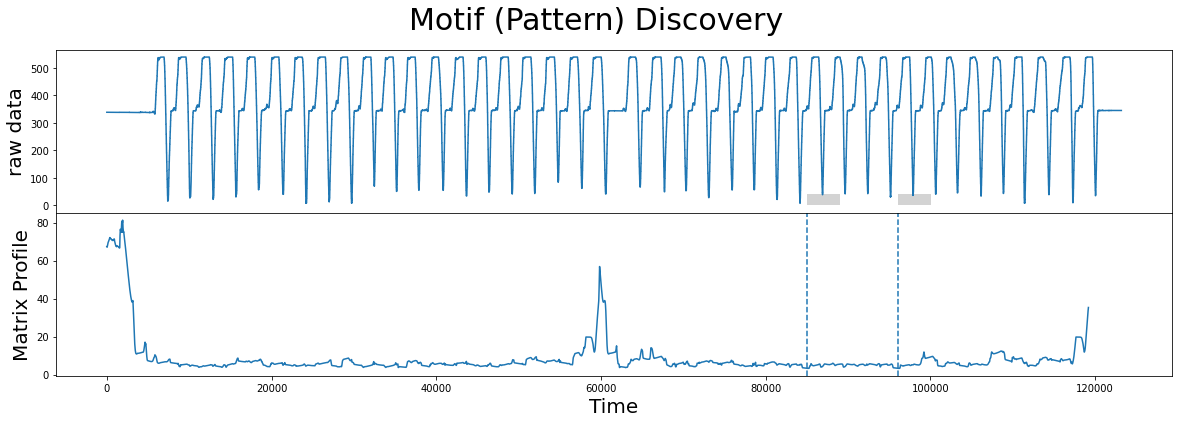
\includegraphics[scale=0.40]{images/Motif (Pattern) Discovery.png}
\caption{Motif (Pattern) Discovery}
\label{Motif}
\end{figure}
According to the documentation XXX, to select a complete cycle, choose the lowest point in the Matrix profile, then add the rough length of the pattern to create the stand and endpoint of the cycle.

Requiring the knowledge of the cycle length prior to running the program highlighted a major problem with stumpy. This problem means that the stumpy library cannot be used if the engineer does not know the cycle length they are after. 
\begin{python}
length = 4000
mp = stumpy.stump(datasetA['mm'], length)

\end{python}

\begin{figure}
\centering
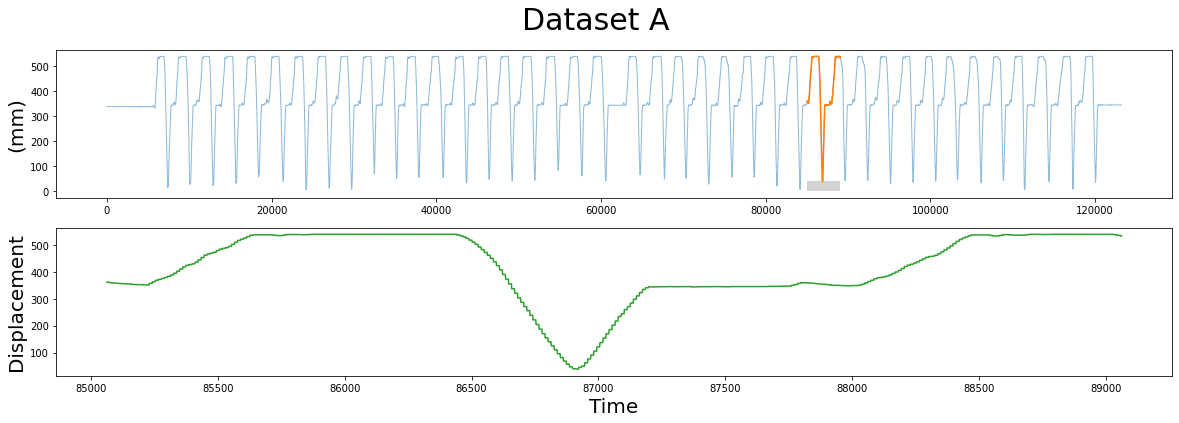
\includegraphics[scale=0.40]{images/DatasetA.png}
\caption{Motif (Pattern) Discovery}
\label{Stumpy Cycle selected}
\end{figure}

\subsection{pyts}
``pyts" is a Python package dedicated to time series classification. It aims to make time series classification easily accessible by providing preprocessing and utility tools, and implementations of several time series classification algorithms. The package comes up with many unit tests and continuous integration ensures new code integration and backward compatibility. The package is distributed under the 3-clause BSD license." \cite{JMLR:v21:19-763}

Throughout researching and testing the tool to see its application, unfortunately, it does not fit the requirements. `pyst' library uses machine learning requiring training samples before running the actual time series data. Under the methodology of the report, no training samples are provided. The function has to find `a representative cycle' with only 1 dataset. `pyst' library fails to do so even if it markets itself as pattern recognition and is confirmed from paper \cite{DBLP:journals/corr/abs-2104-07406}.

\subsection{matrixprofile}

Here is another library based on the z-normalized Euclidean distance papers \cite{zhu_imamura_nikovski_keogh_2017}. 
``MatrixProfile is a Python 3 library, brought to you by the Matrix Profile Foundation, for mining time series data. The Matrix Profile is a novel data structure with corresponding algorithms (stomp, regimes, motifs, etc.) developed by the Keogh and Mueen research groups at UC-Riverside and the University of New Mexico. The goal of this library is to make these algorithms accessible to both the novice and expert through standardization of core concepts, a simplistic API, and sensible default parameter values." \cite{Van_Benschoten2020} 

Unfortunately, at the time of this report, Python 3.10 is not supported. Stopping the author from using the datasets for this library. Fortunately the article \cite{Van_Benschoten2020} provides Figure \ref{matrixTable} of the results from a NYC taxi dataset. Results seem promising for the report with an interesting automatic Discord identifier. Discord is defined as "A time series discord indicates a subsequence with the maximum distance to its neighbor in the given time series data, which means abnormal or unusual data trends."\cite{woodbridge_wilson_rintoul_goldstein_2015}

\begin{figure}
\centering
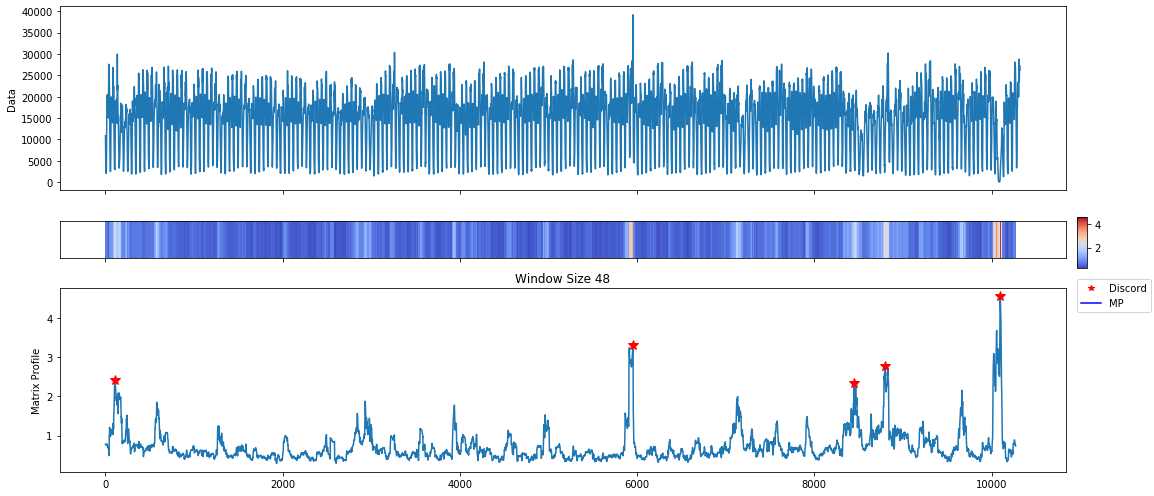
\includegraphics[scale=0.40]{images/examples_NYC_Taxis_8_2.png}
\caption{matrixTable}
\label{matrixTable}
\end{figure}

\subsection{tslearn}
tslearn is another library based on the Scikit-learn platform. A trendy Python package for machine learning. Unfortunately, this library has the same issue as matrixprofile. It relies on training data for the AI to practice before running through the main dataset. No training data is allowed in the report's case, making the tslearn library unsuitable.  


\chapter{Methodology}
\section{Software Considerations}

\raggedright
In the process of software selection, multiple evaluations needed to take place; Access to licensing, the time required to learn the software to an acceptable degree, software feature flexibility, pricing. 

\subsubsection{Matlab}

Matlab was in careful consideration to be the mathematical tool used to generate the graphs and run Autocorrelation. Unfortunately, due to licensing issues and multiple versions available made this process very time-consuming. The last issue was the learning curve was very steep requiring a lot of hours to get little in added benefit.

\subsubsection{Python}

Python was also in careful considering for a mathematical tool. Here the learning curve was easier and with the huge range of tutorials and documentation online, made this the program of choice. Another selling point was the importing of Libraries, using statsmodel allowed me to implement autocorrelation and other statistical features without having to manually code them yourself. Meaning quickly you could get a script up to speed.

\subsubsection{Diadem}

The last software in consideration was Diadem, used to help engineers accelerate the post-processing of measurement data. Designed for large datasets, this would be excellent choice. The only reason Diadem could not other throw Python was the flexibility and open-source of python. Allowing for this skill to be applied in other areas. 

\section{Libraries used}
\subsubsection{Matplotlib}
``Matplotlib is a comprehensive library for creating static, animated, and interactive visualizations in Python. Matplotlib makes easy things easy and hard things possible." \cite{matplotlib}

This library was originaly produced by John D. Hunder American neurobiologist, to provide a a MATLAB-like interface. 
This library is the backbone of the authors script. All data visualisation graphs are produced using this library. Code refers to matplotlib as plt

\subsubsection{NumPy}

NumPy, is another famous open source library created in 2006. Used in a variety of fields of STEM, from engineering to science and mathematics. ``It’s the universal standard for working with numerical data in Python, and it’s at the core of the scientific Python and PyData ecosystems." 

Used by beginners coders to advanced engineers in R\&D. The API is used in depth with most  data science and scientific Python packages but most importantly for us, Matplotlib and pandas. 

The NumPy API is used extensively in Pandas, SciPy, Matplotlib, scikit-learn, scikit-image and most other data science and scientific Python packages.

For this report, NumPy is used in, creating NumPy arrays, mathematical function sum \cite{mhvk} and average and functions. These Numpy arrays are used instead of standard Python lists as they perform better in speed and and more compact. 

\subsubsection{Pandas}

``Flexible and powerful data analysis / manipulation library for Python, providing labeled data structures similar to R data.frame objects, statistical functions, and much more" \cite{pandas}

Pandas in the code are refered to as the standardised name of pd. The sole purpose of this library in this technical report is to import and read the excel data using ``pd.read\_csv".

\subsubsection{Scripy}

Scripy, developed in 2010 by Jonas Melian. ``The main tool of this package is the shell.Run() class which lets to run system commands in the same shell. It works well with pipes and pass the shell variables." \cite{Scripy}.  

In this script it is only used to assist in down sampling the signal data. 
``signal = scipy.signal.resample(signal,123200)" 

\subsubsection{Statsmodels}

``Statsmodels is a Python module that provides classes and functions for the estimation of many different statistical models, as well as for conducting statistical tests, and statistical data exploration. An extensive list of result statistics are available for each estimator. The results are tested against existing statistical packages to ensure that they are correct." statsmodel
The technical report is based on this one library, as it does the mathematical formulas and statistics for autocorrelation in a few lines of code 

\section{Script structure}
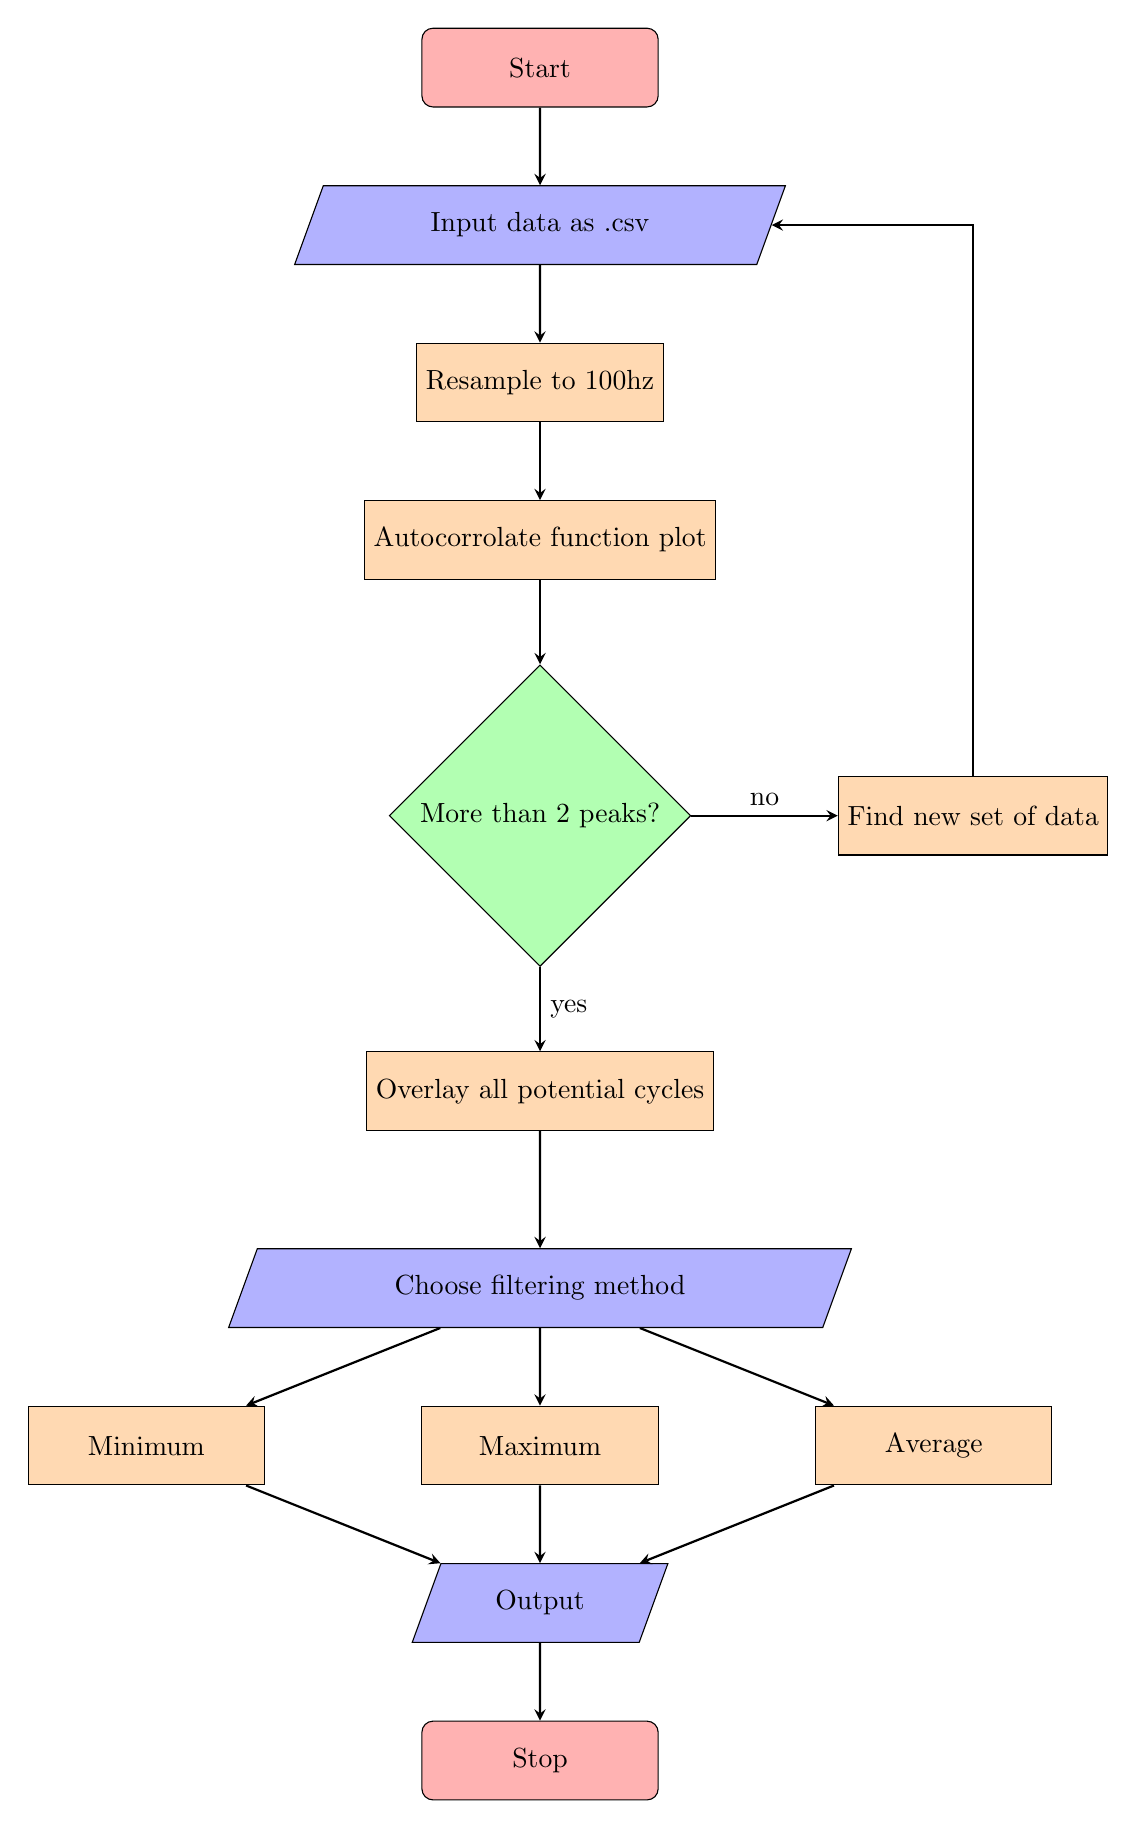
\begin{tikzpicture}[node distance=2cm]

\node (start) [startstop] {Start};

\node (in1) [io, below of=start] {Input data as .csv};

\node (in2) [process, below of=in1] {Resample to 100hz};

\node (pro1) [process, below of=in2] {Autocorrolate function plot};

\node (dec1) [decision, below of=pro1, yshift=-1.5cm] {More than 2 peaks?};

\node (pro2a) [process, below of=dec1, yshift=-1.5cm] {Overlay all potential cycles};
\node (pro2b) [process, right of=dec1, xshift=3.5cm] {Find new set of data};
\node (dec2) [io, below of=pro2a, yshift=-0.5cm] {Choose filtering method};

\node (min) [process, below of=dec2, xshift=-5cm] {Minimum};
\node (max) [process, below of=dec2, xshift=0cm] {Maximum};
\node (ave) [process, below of=dec2, xshift=5cm] {Average};

\node (output) [io, below of=max] {Output};
\node (stop) [startstop, below of=output] {Stop};

\draw [arrow] (start) -- (in1);
\draw [arrow] (in1) -- (in2);
\draw [arrow] (in2) -- (pro1);
\draw [arrow] (pro1) -- (dec1);
\draw [arrow] (dec1) -- node[anchor=south] {no} (pro2b);
\draw [arrow] (dec1) -- node[anchor=west] {yes} (pro2a);
\draw [arrow] (pro2a) -- (dec2);
\draw [arrow] (pro2b) |- (in1);
\draw [arrow] (dec2) -- (min);
\draw [arrow] (dec2) -- (max);
\draw [arrow] (dec2) -- (ave);

\draw [arrow] (min) -- (output);
\draw [arrow] (max) -- (output);
\draw [arrow] (ave) -- (output);

\draw [arrow] (output) -- (stop);


\end{tikzpicture}





\chapter{Results and Analysis}
 \raggedright
\section{Autocorrelation implementation}
The Author's code starts here. How do we implement Autocorrelation using statsmodel library?
Firstly import acf function from statsmodel library insuring it is previously downloaded onto the computer \cite{statsmodel}. Code and print results seen on Figure \ref{a} explain how to import the library as well as calling the function with our dataset (variable `signal'). 

\begin{python}
from statsmodels.tsa.stattools import acf
#Autocorrelate the signal and plot
#signal is the variable with all the raw data
acorr = acf(signal, nlags=(len(signal)))
plt.plot(acorr)
\end{python}

\begin{figure}[ht]
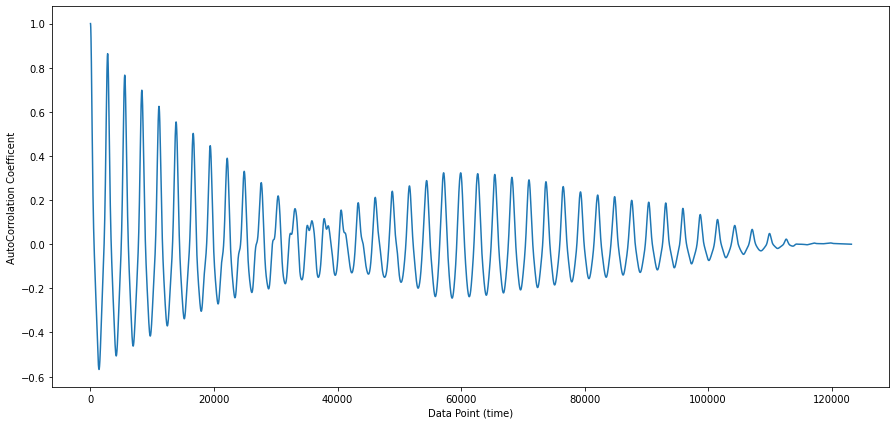
\includegraphics[scale=0.45]{images/autocorrolationCoefficent.png}
\caption{Output}
\label{a}
\end{figure}
The number of lags is equal to the total number of datapoints in plot \ref{a}.
Every peak is a point where the function found a correlation i.e pattern. This explains why at datapoint zero the coefficient of autocorrelation is 1 (100\%) as the script has not had enough time to shift itself by $n$ lags.
The next step is to extract the sections that have relatively high autocorrelation coefficient. This is done by recording all datapoints `peaks'.The process of peaks in the next step can create limitations we will talk about in section \ref{limitation}.


\begin{python}
peak_points = scipy.signal.find_peaks(acorr, height=0.1,prominence=0.2)
plt.ylabel('AutoCorrolation Coefficent')
plt.xlabel('time (datapoints)')
plt.plot(acorr)
plt.plot(peak_points[0],peak_points[1]['peak_heights'],'rx') 
#rx = crosses
\end{python}

\begin{figure}[ht]

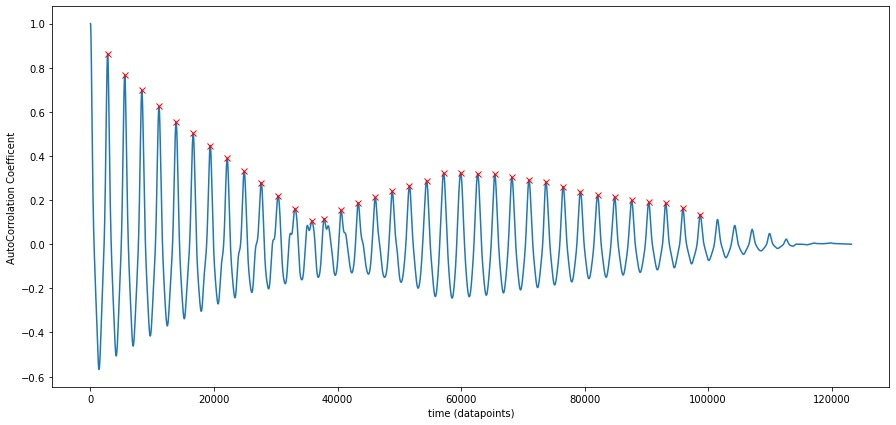
\includegraphics[scale=0.45]{autocorrolationCoefficentWithPeaks.jpg}
\caption{Output}
\label{autocorrolaiton with peaks}
\end{figure}

``peak\_points" array produces a list where in the 123,200 total datapoints the correlation is taking place. In other words, each value in ‘peaks’ array represents a pattern. The next step is to join 2 adjacent peaks to create a start and end of a cycle. This was done using python's built in zip() function. The zip() function returns a zip object, which is an iterator of tuples where the first item in each passed iterator is paired together, and then the second item in each passed iterator are paired together etc.\cite{defZip}. Code in \ref{Paired List} sampled from \cite{paiedList}.

\begin{figure}[ht]
\centering

\begin{python}
"""Creating the timestamps from the peaks""" 
#using zip() + list slicing 
#to perform pair iteration in list
timestamps = list(zip(peaks, peaks[1:] + peaks[:1]))
print("Total cycles",len(timestamps))
# printing result
print ("The pair list is : " + str(timestamps))
\end{python}

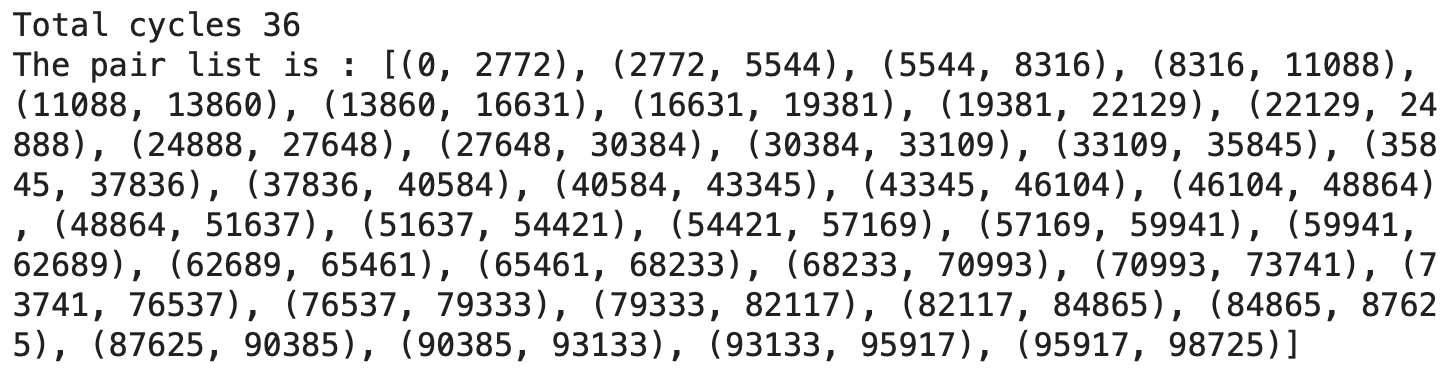
\includegraphics[scale=0.5]{images/arrayPeaks.png}
\caption{Paired List}
\label{Paired List}
\end{figure}

As you can see in figure \ref{Paired List}, we have converted the 37 
`crosses' into 36 cycles with start and end timestamps. List `timestamps' plotted shown on fig \ref{OverlayedCycles}.


\section{Filtering} \label{filtering}
Back to the initial objective, ``Identify a Representative cycle within the larger data set". Next step is deciding which cycle we should pick from the 36 cycles identified. 
\begin{figure}[ht]

\begin{python}
for cycle in cycles_plot:
    plt.plot(cycle)
\end{python}

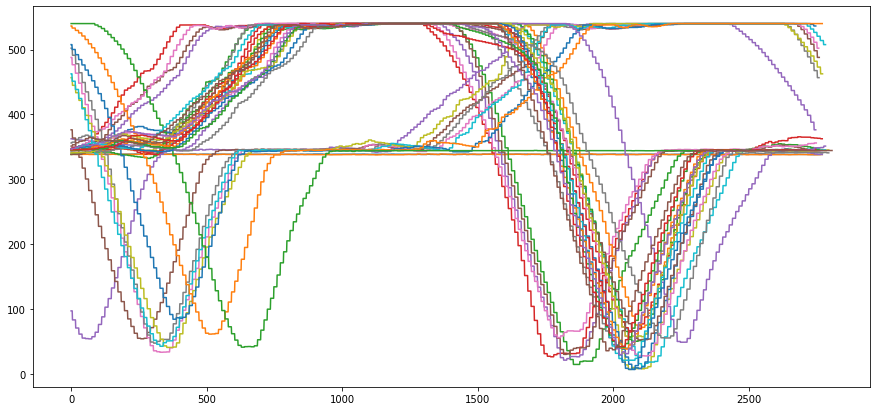
\includegraphics[scale=0.45]{images/cyclesOverlayed.png}
\caption{OverlayedCycles}
\label{OverlayedCycles}
\end{figure}


\subsection{Initial observations:}
\begin{itemize}

    \item Not all the cycles align.
    
    \item All the cycles seem to follow the large dip at time 2000.
    
    \item This dataset seems to have a cap at magnitude of roughly
    500.
    \item Autocorrolation did a good job with this set of data.
    
    \item Some cycles seem longer than others.
    
    \item  The cycles don't all start at the same magnitude 
    
    \item Visually the cycles are very similar.
    
\end{itemize}

\subsection{Maximum peak}
Approach A: filter with maximum peak, lowest trough, largest range 

This approach would give the most extreme cycles. While it is a "...Representative cycle...". It isn't the closest to the "average"

\begin{python}
listforMax=[]

for i in cycles_plot:
    listforMax.append(max(i))    
    
maxIndex = listforMax.index(max(listforMax))

\end{python}

The `for loop' finds the maximum value for each cycle in cycles\_plot then adds it to `listforMax'. Once the loop finishes, it has 36 values, one maximum value for each cycle. If we want to select the cycle with the largest value, variable `maxIndex', holds the index value of this cycle. In our case it is index nº 4.

\subsection{Lowest trough}

\begin{python}
listforMin=[]

for i in cycles_plot:
    listforMin.append(min(i))
    
minIndex = listforMin.index(min(listforMin))

\end{python}

The `for loop' finds the minimum value for each cycle in `cycles\_plot' and then adds it to `listforMin'. Once the loop finishes it has 36 values, one minimum value for each cycle. If we want to select the cycle with the lowest value, variable `minIndex' holds the index value of this cycle. In our case it is index nº 30.

\subsection{Average}
After using the mathematical average approach to find the average peak of all the magnitudes of each cycle, we must find the mean of the 36 values. For the purposes of comprehension, assume it gives us a value of 340.2, and then use Python built in method index() to find the cycle number. Unfortunately the mean or average value calculated might not exist in the actual data, giving the script an error. Instead we have to alter this approach and find the closest real value to the theoretical mean. This is an approach: 

\begin{python}
meanList=[]
for i in cycles_plot:

    meanList.append(np.sum(i)/len(i))
\end{python}

Here we have created a list with 36 values, the overall mean magnitude per cycle, giving the length of this list equal to the total number of cycles found from the Autocorrolation function. 
Next is finding the index and closest real value. 
\begin{python}
closest_real_value = min(meanList, key=lambda x:abs(x-np.average(meanList)))
closest_to_av_index = meanList.index(closest_real_value)

print(closest_to_av_index)
\end{python}

Using Python's built in min function, it finds the minimum distance from the ´meanList' to the real value ``np.average(meanList)". \cite{realValue}

The `meanList.Index()' function finds the index of our  ´closest\_real\_value' Giving an output of cycle nº 13.

\subsection{Filtering limitations}
Average, minimum and maximum work in the authors case but everyone's use case is different. Exploring other options like Standard deviations, most common cycle, 25 quarterly could be explored. 
\section{Autocorrelation limitation}\label{limitation}

When the signal data has a greater Randomness the magnitude of the Autocorrelation coefficient is reduced drastically. 

The lower the amount of cycles found, the higher the probability that the cycle selected is not ``...Representative...". 

\begin{figure}[ht]
\centering
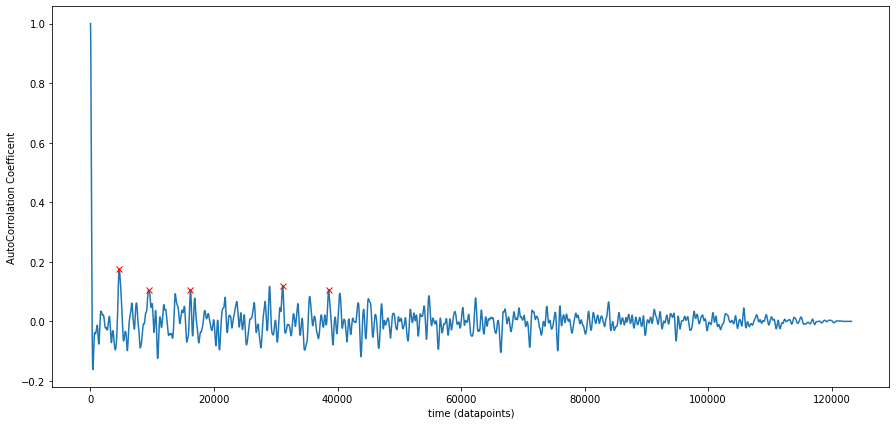
\includegraphics[scale=0.40]{images/autocorrolationBadCoefficentWithPeaks.png}
\caption{Limit Testing B}
\label{LimitA}
\end{figure}

Stress testing `acf' function with dataset B, the displacement steering cylinder dataset has a higher randomness compared to the dataset A used in the rest of the report. This translates to a decrease in total cycles found. The amount of cycles identified went from 36 to 5, 86\% decrease. 
This can be justified as the steering cylinder has a lot of feedback from the machine's steer over rocks and uneven terrain unlike the lift or tilt cylinder.

\begin{figure}[ht]
\centering
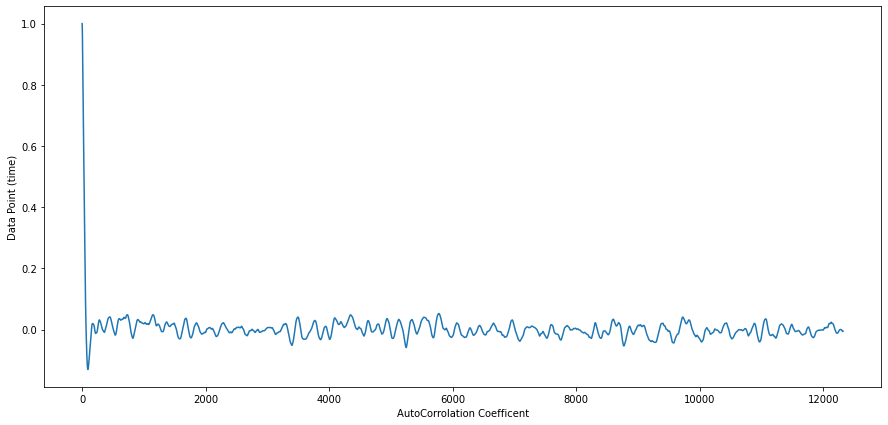
\includegraphics[scale=0.40]{images/limitTestB.png}
\caption{Limit Testing C }
\label{LimitB}
\end{figure}
The heaviest stress testing was with dataset C, ref \ref{LimitB}.This data came from a strain gauge force dataset attached to a CAT machine. Here the function failed to correlate a single Dataset. Factors for this result could be 500hz sensor data causing too much noise. Forces by nature are going to be harder to correlate compared to displacement. 

\chapter{Conclusions}
\section{Technical/Commercial Content}

In this day and age, we are receiving ever more data. Unfortunately, raw data is meaningless without the Skills and tools to analyse it.

The Commercial benefit of Autocorrelation is that it saves the company resources. It reduces the time needed to filter through hours of machine data, as the engineers only have to analyse one cycle instead of hundreds. It also facilitates the engineer in identifying micro details in a cycle that would be drowned in hours of data. 

Data science tools are increasing in popularity especially in engineering teams, to assist in large decision. The companies using data science tools range from financial services to AMG Mercedes F1 team in solving their 'porpoising' issue \cite{mercedes}. 

\subsection{Key findings}
The script produced with the Statsmodels ACF function, shows promising results for a method of cycle identification in python. Successfully working with 2 out of the 3 datasets tested against it. Only failing with dataset C, 'Force Strain gauge' seemingly due to the 500hz frequency and high noise related to strain gauges.

Filtering was another hurdle in producing a fully functioning tool using autocorrelation. Three methods were produced with the most complex one being the 'mean' function nonetheless this area is a weak link in the report. More advanced filtering methods could be investigated when narrowing down the group of cycles to one representative cycle. 

\subsection{Recommendations}
For cycle identification the findings suggests that the reader tries out both Statsmodel and Stumpy to see which method fits their specific needs better. 
\subsubsection{Autocorrelation}
For pattern recognition without cycle length knowledge use the tool. If large changes need to be made to the original script, the author recommends extracting the acf function from Statsmodel library instead of editing the whole script. 
An idea that could investigated to improve the tools performance with higher randomness data like Dataset C. Investigate lowering the height constant and changing the prominence value in the peaks function. 

\begin{python}
#Find peak points
peak_points = scipy.signal.find_peaks(acorr, height=0.1,prominence=0.2)
\end{python}

\subsubsection{Stumpy}
If the length of cycle is known, stump function even worked with dataset C, at 500hz, something that the autocorrelation script failed in.
If Stumpy is chosen and reader is having issues with processing time required. Stumpy library offers an accelerated version through a Nvidia GPU version of the STUMP function. Author was unable to test this version due to limited access to a specific brand gpu. 
\begin{python}
import stumpy
mp = stumpy.gpu_stump(df['value'], m=m)  
# Note that you'll need a properly configured NVIDIA GPU for this
\end{python}

Also consider checking the Github page and the documentation as the library can be updated at any moment due with other tutorials and examples due to the open source nature of the library. \cite{law2019stumpy}




\appendix
\chapter{Complete code}
\begin{python}

import matplotlib.pyplot as plt
import numpy as np
import pandas as pd
import scipy
from statsmodels.graphics.tsaplots import plot_acf
from statsmodels.tsa.stattools import acf

#Autocorrelate the signal and plot
plt.figure(figsize=(15,7))
plt.ylabel('AutoCorrolation Coefficent')
plt.xlabel('Data Point (time)')
acorr = acf(signal, nlags=(len(signal)/10))
plt.plot(acorr)

file="STR_ABS_AX_F_COMB_HAND_BANK.CSV"

rawData = pd.read_csv (file, header=11)

signal = rawData["kN"].to_numpy()       
signal = scipy.signal.resample(signal,123200)

plt.figure(figsize=(15,4))
plt.plot(signal)

#Autocorrelate the signal and plot
plt.figure(figsize=(15,7))
plt.ylabel('AutoCorrolation Coefficent')
plt.xlabel('Data Point (time)')
acorr = acf(signal, nlags=(len(signal)/10))
plt.plot(acorr)

#Find peak points
peak_points = scipy.signal.find_peaks(acorr, height=0.1,prominence=0.2)

# peak_points 4D array, 1D = timestamp, , 2D = peak_heights, 3D = left_based, 4D = right_based,

plt.figure(figsize=(15,7))
plt.ylabel('AutoCorrolation Coefficent')
plt.xlabel('time (datapoints)')
plt.plot(acorr)
plt.plot(peak_points[0],peak_points[1]['peak_heights'],'rx') #rx = crosses

peaks = np.append([0],peak_points[0])
len(peaks)

"""Creating the timestamps from the peaks"""
#using zip() + list slicing 
#to perform pair iteration in list
timestamps = list(zip(peaks, peaks[1:] + peaks[:1]))
print("Total cycles",len(timestamps))
# printing result
print ("The pair list is : " + str(timestamps))

#Plot all cycles overlayed

cycles_plot= [] 
for a,b in zip(peaks[:-1],peaks[1:]):
    cycles_plot.append(signal[a:b])
cycles_plot # a 2D list, each element is 1 all the points in 1 cycle
print(type(cycles_plot))
print("There's", len(cycles_plot), "cycles plotted" )

plt.figure(figsize=(15,7))
for cycle in cycles_plot:
    plt.plot(cycle)
    
    
listforMax=[]

for i in cycles_plot:
    listforMax.append(max(i))    
maxIndex = listforMax.index(max(listforMax))

print("max value from list is",max(listforMax))
print("for function max, cycle index is",maxIndex)


listforMin=[]

for i in cycles_plot:
    listforMin.append(min(i))
    
minIndex = listforMin.index(min(listforMin))

print("min value from list is",min(listforMin))
print("for function max, cycle index is",minIndex)

meanList=[]
for i in cycles_plot:

    meanList.append(np.sum(i)/len(i))
    
closest_real_value = min(meanList, key=lambda x:abs(x-np.average(meanList)))
print(closest_real_value)
plt.plot(cycles_plot[13])
closest_to_av_index = meanList.index(closest_real_value)
print(closest_to_av_index)

\end{python}

\printbibliography

\end{document}
